\documentclass[titlepage,a4paper,12pt]{ltjsreport}

\usepackage{luatexja}
\usepackage{amsmath,amsfonts}
\usepackage{amsthm}
\usepackage{bm}
\usepackage[dvipdfmx]{graphicx}
\usepackage{color}
\usepackage{caption}
\usepackage{url}
\usepackage{listings}
\usepackage{abstract}
\usepackage{multicol}
\usepackage{geometry}
\usepackage{here}
\usepackage{tabularx}


\lstset{
    basicstyle={\ttfamily},
    identifierstyle={\small},
    commentstyle={\small},
    keywordstyle={\small\bfseries},
    ndkeywordstyle={\small},
    stringstyle={\small\ttfamily},
    frame={tb},
    breaklines=true,
    columns=fixed,
    basewidth=0.465em,
    numbers=left,
    numberstyle={\scriptsize},
    lineskip=-0.5ex
}


\begin{document}

\leftline{課題7　要求記述}
\rightline{256E0143
三留 慎太郎}

\begin{enumerate}
    \item 概要 \mbox{}\\
    数値$x$と$y$の集合の相関と有意性、$n$組のペアに対する回帰パラメータ$\beta_0$と$\beta_1$を計算し、与えられた見積もり値$x_k$を与えられた際の予測値$y_k$を計算し、それに対する70\%予測区間を計算する。

    \item 詳細\mbox{}\\
    求める値とその計算方法の詳細を以下に示す

    求める順序と値
    \begin{enumerate}
        \item 数値$x$と$y$の集合の相関係数$r_{x,y}$,$r^2$を求める
        \item その相関の有意性$tail\ area$を計算する
        \item n組のペアに対する線形回帰パラメータ$\beta_0$, $\beta_1$を計算する
        \item パラメータを用いて与えられた$x_k$に対する予測値$y_k$を計算する
        \item 70\%の予測範囲Rangeを計算する
        \item 見積もり値に対する予測区間の上限UPIと下限LPIを計算する\\
    \end{enumerate}
    

    ここで、相関有意性$tail\ area$の計算手順は以下の通り。

    \begin{enumerate}
        \item $x$の値を計算する
        
        \[
        x = \frac{\left\lvert r_{x,y} \right\rvert \sqrt{n-2} }{\sqrt{1-{r_{x,y}}^2}}
        \]
        ここで、$r_{x,y}$は相関、nはデータ点数

        \item 自由度n-2のt分布を0から$x$まで数値積分して確率pを求める
        \item 1-2pとしてテイルエリアを計算する\\
    \end{enumerate}

    
    ここで、予測区間を計算するには以下のステップを用いる
    \begin{enumerate}
        \item 70\%区間の範囲Rangeを計算する
        \[
        Range = t(0.35, dof)\sigma \sqrt{1 + \frac{1}{n} + \frac{(x_k - x_{avg})^2}{\sum_{n = 1}^{n} (x_i - x_{avg})^2} } 
        \]
        ここで、nはデータ点数、$t(0.35,\ dof)$は自由度n-2、p=0.35のt分布のxの値であり、標準偏差\sigma は以下の計算式で計算できる。
        \[
        \sigma = \sqrt{(\frac{1}{n-2} \sum_{i = 1}^{n} (y_i - \beta _0 - \beta _1x_i)^2 )} 
        \]

        \item UPIを$y_k +$ Rangeとして計算する
        \item LPIを$y_k -$ Rangeとして計算する
    \end{enumerate}

    \item 入力\mbox{}\\
    
    \begin{itemize}
        \item データの入力：csvファイル入力
        \item 入力ファイル：図\ref{data}のように、カンマ区切りの表形式で表現する。\\
        
        \begin{figure}[H]
            \centering
            
\includegraphics[width=0.4\textwidth]{../picture/課題7/data.png}
            \caption{入力データ}
            \label{data}
        \end{figure}
        
        \item 実行時の入力：コマンドラインに以下の形式で入力\\
        　java プログラム名 実数値入力ファイル名 見積もり値
        \item 実行時入力例：java Program7 data\_program7.csv 386\\
                
    \end{itemize}


    \item 出力\mbox{}\\
    \begin{itemize}
        \item 出力方法：コマンドライン出力
        \item 出力する値：$r_{x,y},r^2,tail\ area,\beta_0,\beta_1,y_k,Range,UPI(70\%),LPI(70\%)$
        \item 精度：有効桁通りに表示する。ただし有効桁が11桁以上ある場合、11桁目を四捨五入し、10桁で表示する。なお、tail areaの値については、値が0.0001より小さい場合に限り上記の表示規則に加えて指数表示を用いる。
        \item 出力例：図\ref{kitaiti}のように出力する値をそれぞれ改行して表示する。
        
        \begin{figure}[H]
            \centering
            
\includegraphics[width=0.4\textwidth]{../picture/課題7/kitaiti.png}
            \caption{出力例}
            \label{kitaiti}
        \end{figure}

    \end{itemize}


    \item テスト\mbox{}\\
    以下の4つケースでテストを行う。
    \begin{itemize}
        \item テスト1：表\ref{testdata1}の見積りプロキシ規模と追加・修正の実績値を使用する。見積り値および予測区間を作成する際に、見積りプロキシ規模 xk = 386 を使用する。
        \item テスト2：表\ref{testdata1}の見積りプロキシ規模と開発時間の実績値を使用する。見積り値および予測区間を作成する際に、見積りプロキシ規模 xk = 386使用する。
        \item テスト3：表\ref{testdata2}に示すプログラム3～6の、推定プロキシ・サイズと実際の追加サイズおよび変更サイズを使用する。プログラム7推定プロキシ・サイズxk = 47.6を使用する。
        \item テスト4：表\ref{testdata2}に示すプログラム3～6の、見積りプロキシ規模と開発時間の実績値を使用する。プログラム7の見積りプロキシ規模xk = 47.6を使用する。
    \end{itemize}

    \begin{table}[H]
        \centering
        \caption{テストデータ1}
        \label{testdata1}
        \begin{tabularx}{\textwidth}{|c|X|X|X|c|}
            \hline
            プログラム番号 & 見積りプロキシ規模 & 追加・修正規模の計画値 & 追加・修正規模の実績値 & 開発時間の実績値 \\
            \hline
            1 & 130 & 163 & 186 & 15.0 \\
            2 & 650 & 765 & 699 & 69.9 \\
            3 & 99 & 141 & 132 & 6.5 \\
            4 & 150 & 166 & 272 & 22.4 \\
            5 & 128 & 137 & 291 & 28.4 \\
            6 & 302 & 355 & 331 & 65.9 \\
            7 & 95 & 136 & 199 & 19.4 \\
            8 & 945 & 1206 & 1890 & 198.7 \\
            9 & 368 & 433 & 788 & 38.8 \\
            10 & 961 & 1130 & 1601 & 138.2 \\
            \hline
        \end{tabularx}
    \end{table}
    
    \begin{table}[H]
        \centering
        \caption{テストデータ2（課題3～6）}
        \label{testdata2}
        \begin{tabular}{|c|c|c|c|}
            \hline
            課題番号 & 見積りプロキシ規模 & 追加・修正規模の実績値 & 開発時間の実績値 \\
            \hline
            3 & 77.6 & 118 & 577 \\
            4 & 66 & 45 & 286 \\
            5 & 44.7 & 76 & 358 \\
            6 & 45.7 & 49 & 330 \\
            \hline
        \end{tabular}
    \end{table}

    テスト1-4の期待値を図\ref{kitaiti_expected}-図\ref{kitaiti4}に示す。
    
    \begin{figure}[H]
        \centering
        
\includegraphics[width=0.8\textwidth]{../picture/課題7/kitaiti.png}
        \caption{期待値（テスト1）}
        \label{kitaiti_expected}
    \end{figure}

    \begin{figure}[H]
        \centering
        
\includegraphics[width=0.8\textwidth]{../picture/課題7/kitaiti2.png}
        \caption{期待値（テスト2）}
        \label{kitaiti2}
    \end{figure}

    \begin{figure}[H]
        \centering
        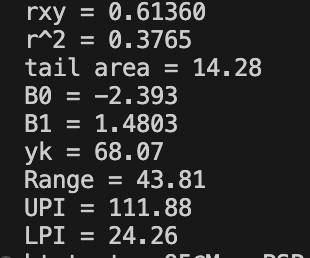
\includegraphics[width=0.8\textwidth]{../picture/課題7/kitaiti3.png}
        \caption{期待値（テスト3）}
        \label{kitaiti3}
    \end{figure}

    \begin{figure}[H]
        \centering
        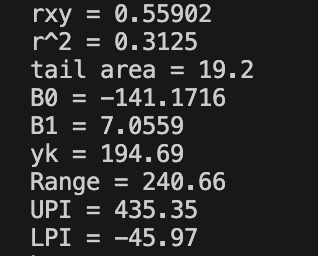
\includegraphics[width=0.8\textwidth]{../picture/課題7/kitaiti4.png}
        \caption{期待値（テスト4）}
        \label{kitaiti4}
    \end{figure}

\end{enumerate}

\end{document}